\subsection{Du quadrilatère au parallélogramme}

	\begin{myprops}
		\begin{itemize}
			\item \textbf{Si} un quadrilatère a ses \kw{côtés opposés parallèles} \textbf{alors} c'est un parallélogramme.
			\item \textbf{Si} un quadrilatère (non croisé) a ses \kw{côtés opposés de même longueur} \textbf{alors} c'est un parallélogramme.
			\item \textbf{Si} un quadrilatère (non croisé) a \kw{deux côtés opposés parallèles et de même longueur} \textbf{alors} c'est un parallélogramme.
			
			\item \textbf{Si} un quadrilatère a ses \kw{diagonales qui se coupent en leur milieu} \textbf{alors} c'est un parallélogramme.
			
		\end{itemize}
	\end{myprops}

	\begin{myex}
		Déterminer la nature du quadrilatère ABCD sachant que $(AB)//(CD)$.
		
			\begin{center}
				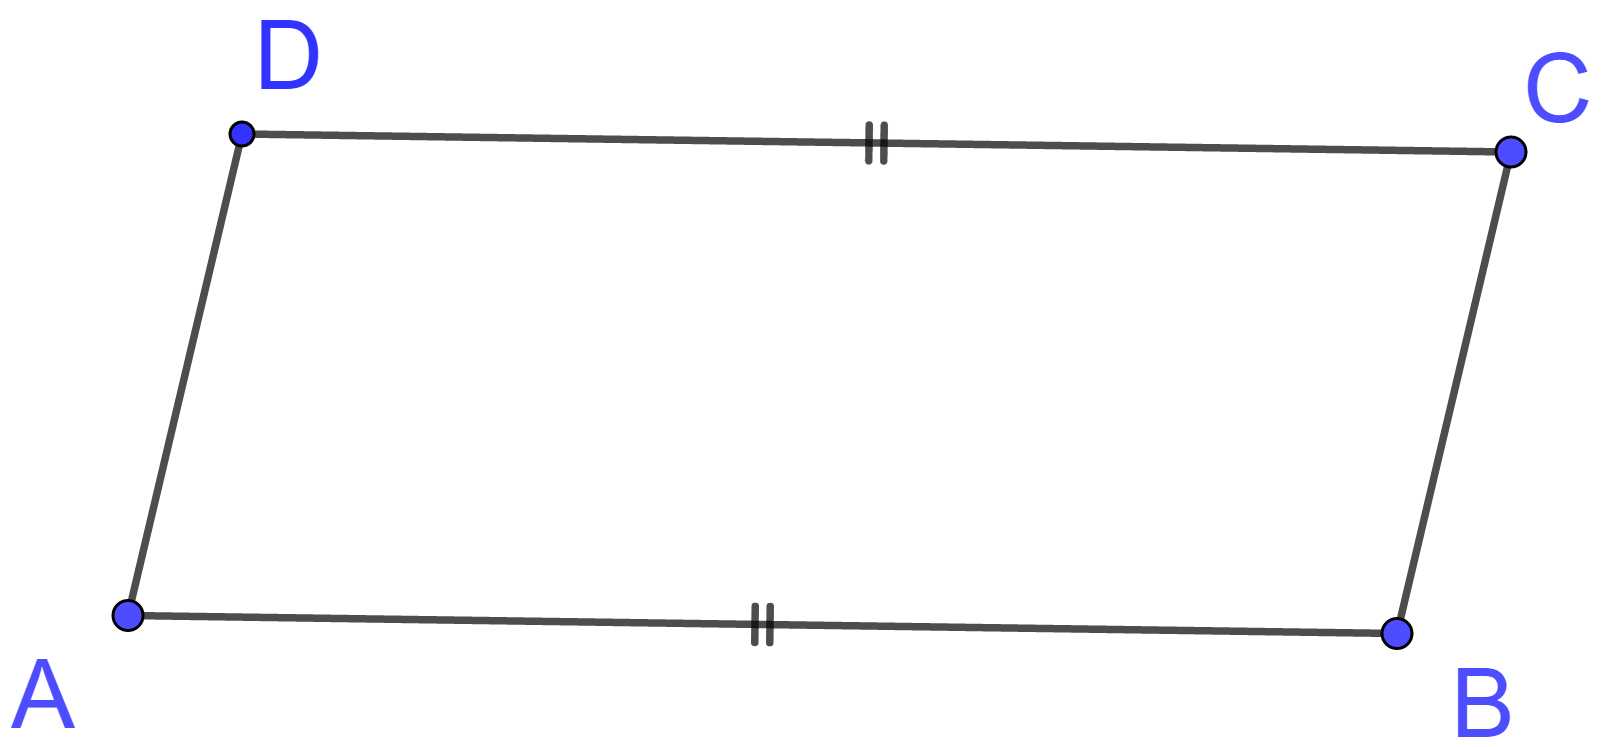
\includegraphics[scale=0.15]{demo1}
			\end{center}
			
			Je sais que $(AB)//(CD)$ et $AB=CD$.
			
			Or si un quadrilatère (non croisé) a deux côtés opposés parallèles et de même longueur alors c'est un parallélogramme.
			
			Donc ABCD est un parallélogramme.
			
		
	\end{myex}


\subsection{Du parallélogramme aux parallélogrammes particuliers}

	\begin{myprop}
		
		\begin{itemize}
			\item \textbf{Si} un parallélogramme a \kw{deux côtés consécutifs perpendiculaires} \textbf{alors} c'est un rectangle.
			\item \textbf{Si} un parallélogramme a \kw{ses diagonales de même longueur} \textbf{alors} c'est un rectangle.
		\end{itemize}
	\end{myprop}


	\begin{myex}
		Déterminer la nature du parallélogramme ABCD.
		
		\begin{center}
			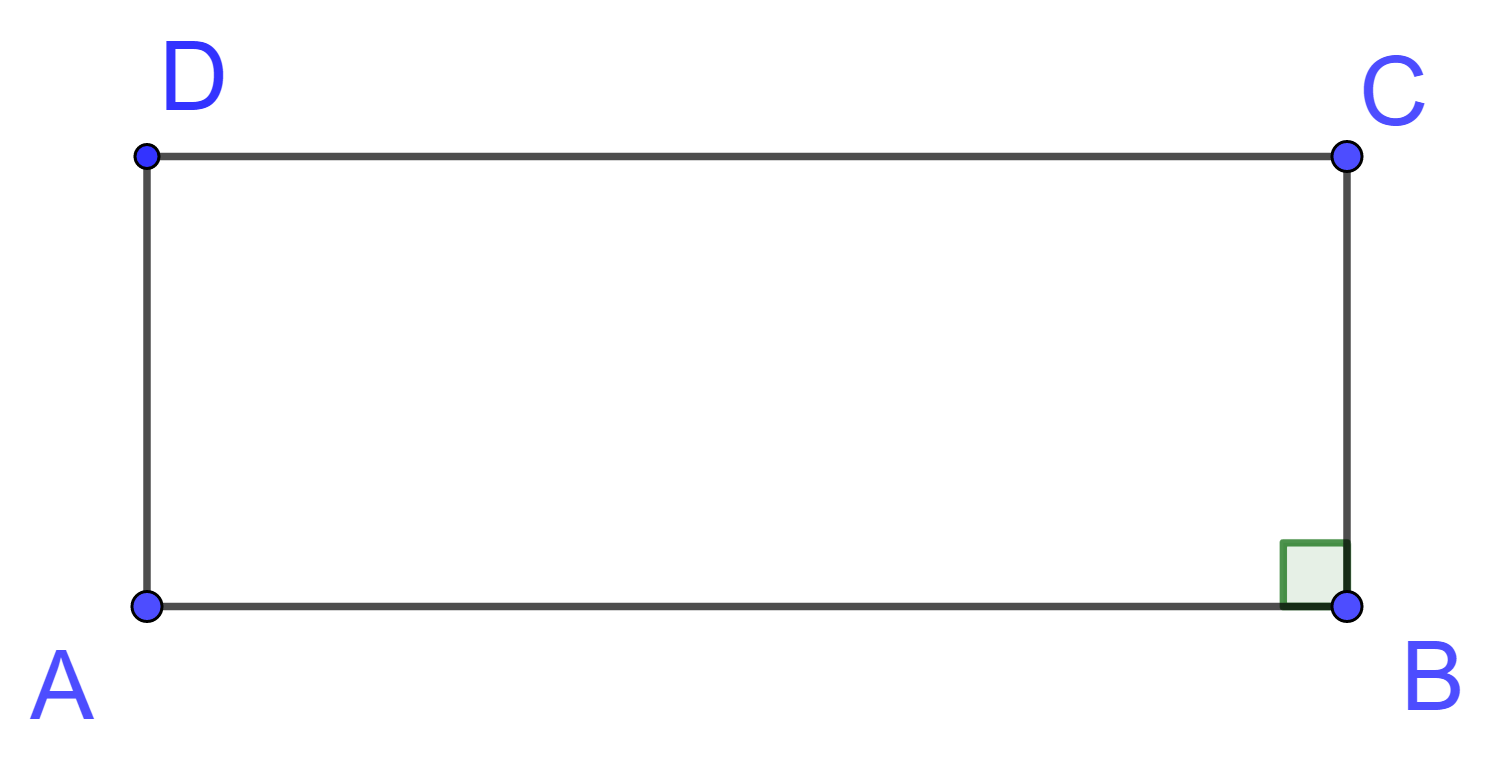
\includegraphics[scale=0.15]{demo2}
		\end{center}
		
		Je sais que ABCD est un parallélogramme et $(AB) \perp (BC)$.
		
		Or si un parallélogramme a deux côtés consécutifs perpendiculaires alors c'est un rectangle.
		
		Donc ABCD est un rectangle.
		
		
	\end{myex}

	\begin{myprops}
		\begin{itemize}
			\item \textbf{Si} un parallélogramme a \kw{deux côtés consécutifs de même longueur} \textbf{alors} c'est un losange.
			\item \textbf{Si} un parallélogramme a \kw{ses diagonales perpendiculaires} \textbf{alors} c'est un losange.
		\end{itemize}
		
	\end{myprops}

	\begin{myex}
		Déterminer la nature du parallélogramme ABCD.
		
		\begin{center}
			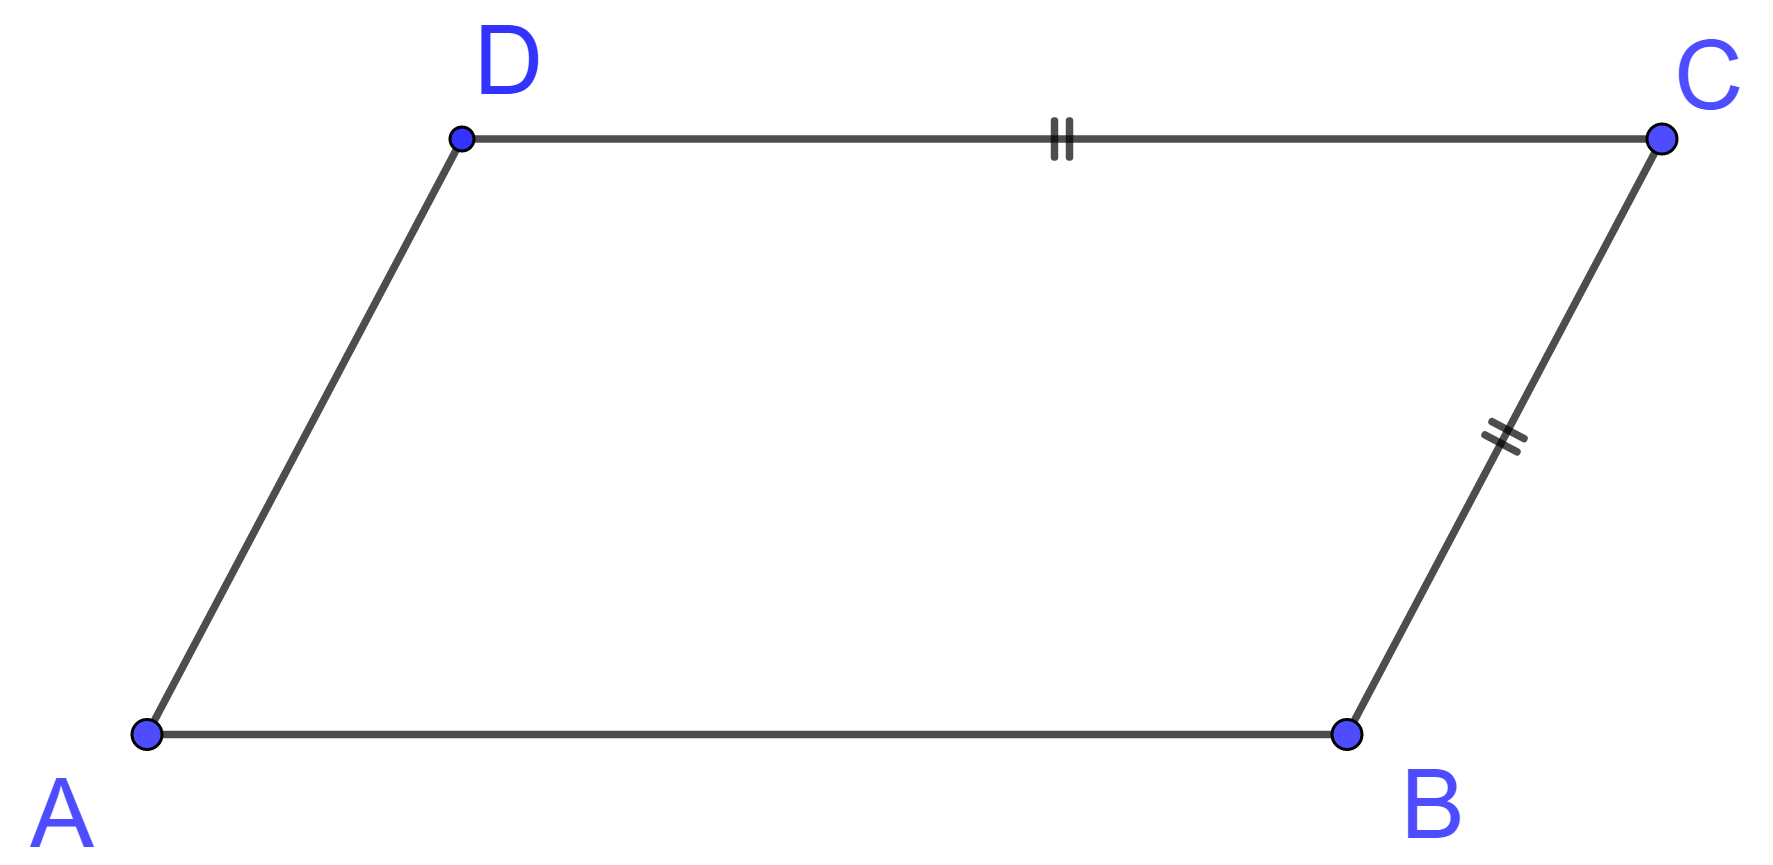
\includegraphics[scale=0.15]{demo3}
		\end{center}
		
		Je sais que ABCD est un parallélogramme et $BC=CD$.
		
		Or si un parallélogramme a deux côtés consécutifs de même longueur alors c'est un losange.
		
		Donc ABCD est un losange.
		
		
	\end{myex}

\newpage

	\begin{myprop}
		\textbf{Si} un quadrilatère est \kw{à la fois un losange et un rectangle} \textbf{alors} c'est un carré.
	\end{myprop}


	
%	\begin{myprop}
%		\begin{itemize}
%			\item \textbf{Si} un parallélogramme a \kw{deux côtés consécutifs de même longueur et perpendiculaires}   \textbf{alors} c'est un carré.
%			\item \textbf{Si} un parallélogramme a \kw{ses diagonales perpendiculaires et de même longueur} \textbf{alors} c'est un losange.
%		\end{itemize}
%	\end{myprop}


	\begin{myex}
		Déterminer la nature du quadrilatère ABCD.
		
		\begin{center}
			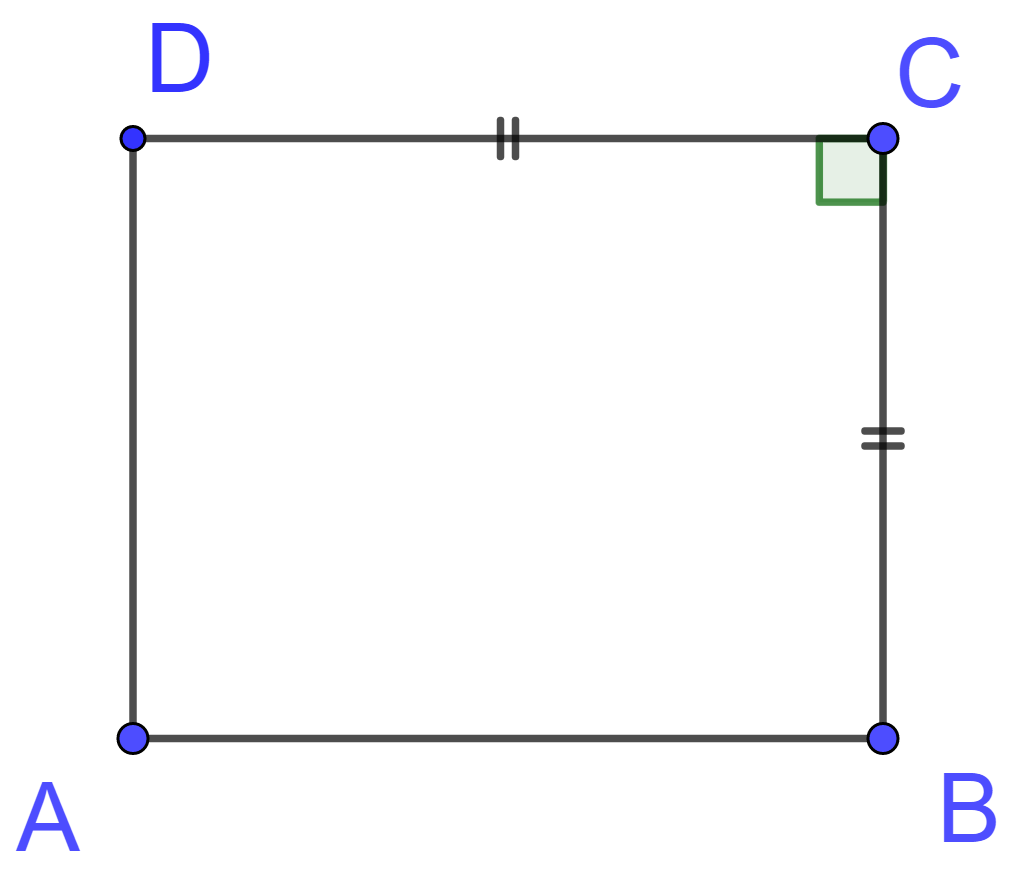
\includegraphics[scale=0.18]{demo4}
		\end{center}
		
		Je sais que ABCD est un parallélogramme et $BC=CD$.
		
		Or si un parallélogramme a deux côtés consécutifs de même longueur alors c'est un losange.
		
		Donc ABCD est un losange.\\
		
		Je sais que ABCD est un parallélogramme et $(BC) \perp (CD)$.
		
		Or si un parallélogramme a deux côtés consécutifs perpendiculaires alors c'est un rectangle.
		
		Donc ABCD est un rectangle.\\
		
		Je sais que ABCD est un losange et ABCD est un rectangle.
		
		Or si un quadrilatère est à la fois un losange et un rectangle alors c'est un carré.
		
		Donc ABCD est un carré.
	\end{myex}